
\documentclass{article}
\setlength{\columnsep}{20pt}
%\usepackage{url}
%\usepackage{algorithmic}
\usepackage[a4paper]{geometry}
\usepackage{datetime}
\usepackage[font=small,labelfont=it]{caption}
\usepackage{graphicx}
\usepackage{mathpazo} % use palatino
\usepackage[scaled]{helvet} % helvetica
\usepackage{microtype}
\usepackage{amsmath}
\usepackage{subfigure}
\usepackage{hyperref}
\usepackage[export]{adjustbox}
\usepackage{multicol}% http://ctan.org/pkg/multicols


% Letterspacing macros
\newcommand{\spacecaps}[1]{\textls[200]{\MakeUppercase{#1}}}
\newcommand{\spacesc}[1]{\textls[50]{\textsc{\MakeLowercase{#1}}}}

\title{\vspace{-2.0cm}\spacecaps{WarInspector: Visual Analytics web application on Arms Transfer}\\ \normalsize \spacesc{Visual Analytics Course Sapienza University of Rome} }

\author{Giuseppe Capaldi 1699498\\ Gianmarco Cariggi}
%\date{\today\\\currenttime}%
\date{\today}

\begin{document}
\maketitle




%%% Big Figure
\begin{figure}[ht!]
\centering
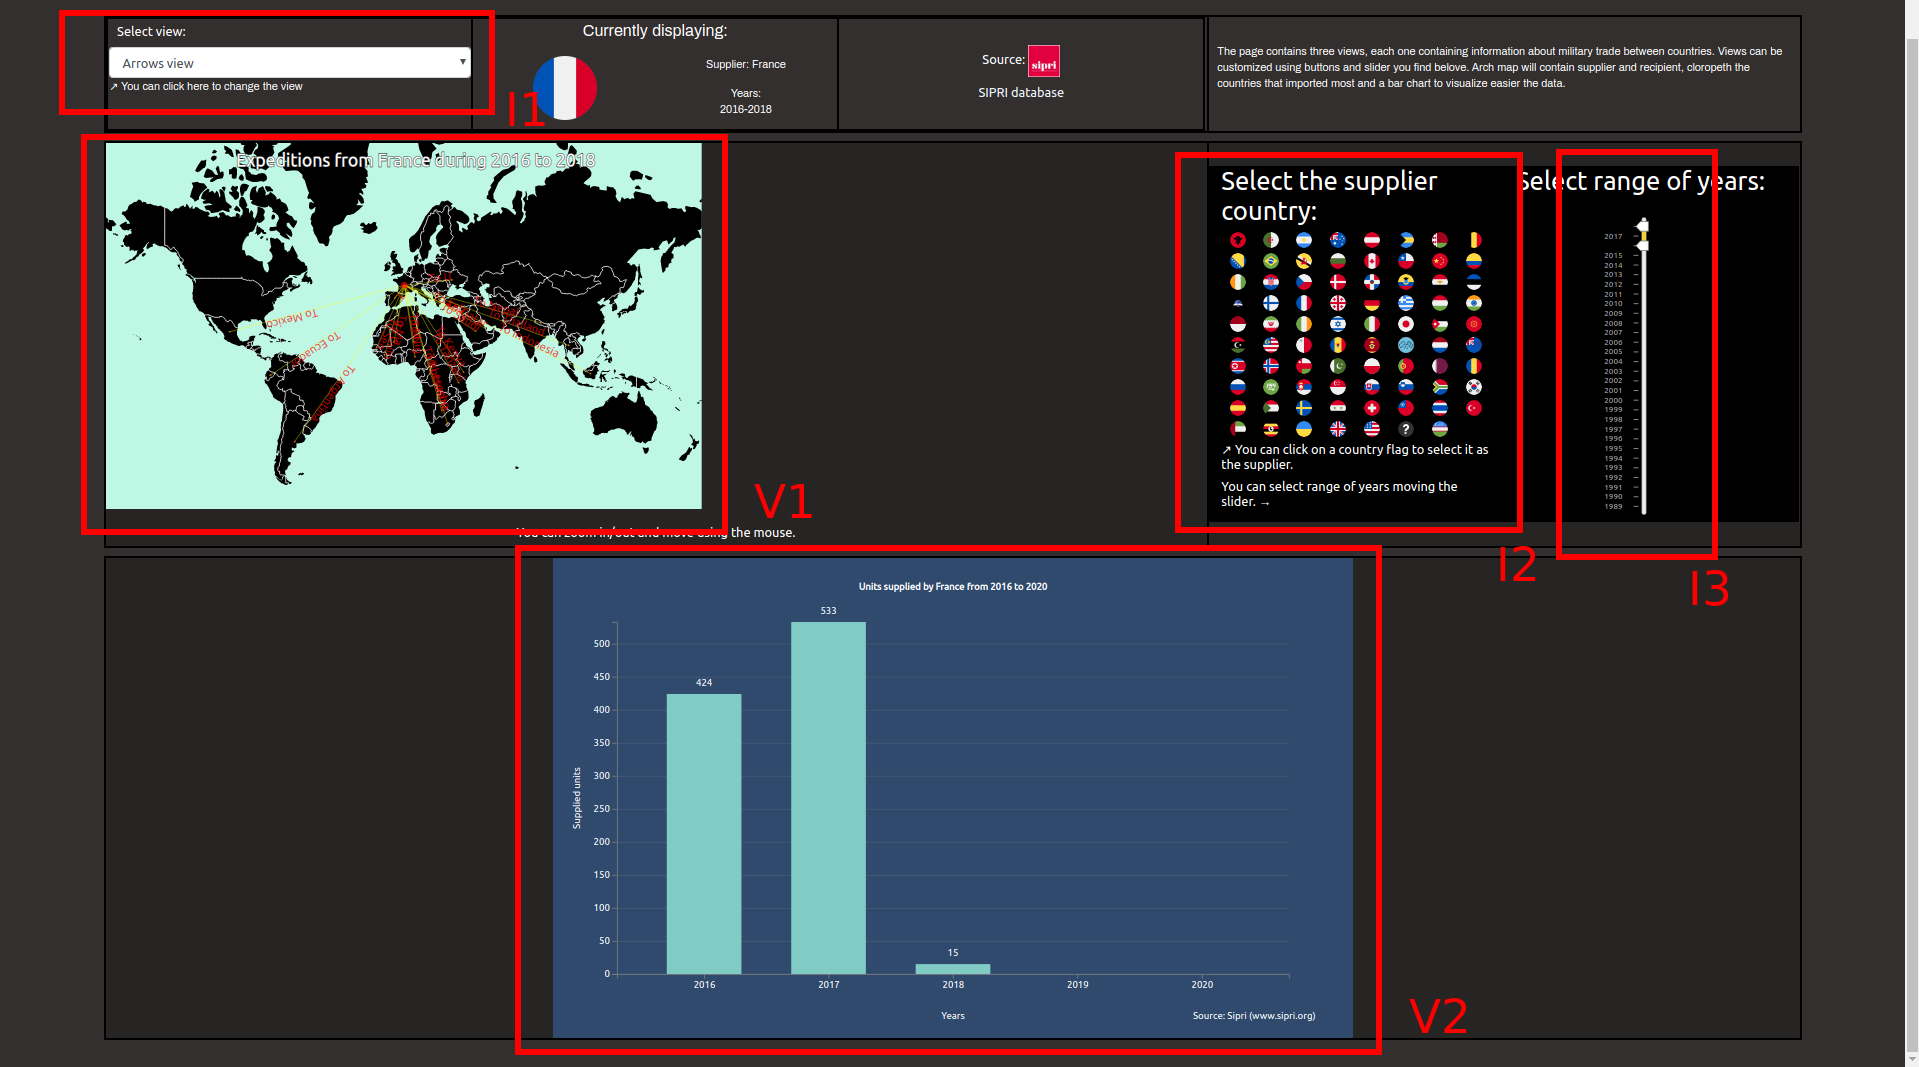
\includegraphics[scale=0.25,center]{fig/va.png}
   \label{fig:va}
    \caption{System interface of the web application homepage. I1, I2, I3 are interactive elements whereas V1, V2 are visual elements. }

\end{figure}
    
    
\begin{abstract}
%
In this report, we present results and design process from "WarMonopoly", an html local page embedding D3.js to visualize some SIPRI (Stockholm International Peace Research Institute) datasets. The page contains user interactive views as barcharts, choropleth map and arc map due to the geographical nature of the data involved. It is present also a scatter plot result of MDS (Multi-Dimensional scaling), computed in python and visualized on the same page, not to preprocess the data but to add new informations to the user. Python program to compute and visualize in real-time MDS depending on user parameters, is hosted on an "Heroku dyno" (a cloud container to host python codes).


%
\end{abstract}

\begin{multicols}{2}

\section{Introduction}
%
In order to offer a data visualization work that would have been interisting in his results, we chose to think of a dataset that could involve the entire planet and containing useful information. Searching the web SIPRI website stood out cause of the possibility it offers to analyze and visualize datasets regarding military trade (from official reports of NATO and every single country which participates to this initiative) among countries. The dataset contains these information: suppliers and recipients, the type and number of weapon systems ordered and delivered, the years of deliveries and the financial value of the deal (but only in some cases). 


We started from this to think of what visual analytics technique would have fit best our purpose and our data.



\section{Dataset}
%


To have a dataset ready to be visualized easily we needed a well formatted file, a CSV (Comma Separated Values) would have been ideal, but the only format offered for our specific dataset of interest (the army transfer database) was RTF (Rich Text Format), that is better to visualize a text due to the presence of text formatting elements, less for storing and visualize a dataset. So we downloaded from: \url{http://armstrade.sipri.org/armstrade/page/trade_register.php} selecting all suppliers and all recipients from 2000 to 2018 (2019 was not present at the time), all weapon system and from supplier register. So after a quick analyis of its content, some Python scripts helped us to reach our CSV file containing a dataset with this format [Table 1]:
\begin{itemize}
\item \textbf{Ordered}: the number of items ordered under the deal
\item \textbf{Weapon model}: the designation of the weapon system concerned
\item \textbf{Weapon category}: description of the weapon system concerned
\item \textbf{Ordered year}: the year the order was placed or, in the case of licensed production, the licence was issued
\item \textbf{Delivered year}: the year or years during which deliveries took place. If no deliveries have yet been made, this field is left blank.
\item \textbf{Delivered num}: the number of items delivered or produced under the deal
\item \textbf{Comments}: any additional information that is known about the deal. This can include the financial value of the deal, what the weapons will ostensibly be used for, whether the weapons are being donated as military aid, and any information on offsets linked to the deal.
 
\end{itemize}



In a second phase in order to draw arrows from a supplier country towards the Recipients we joined the upper dataset with a second one containing only latitude-longitude coordinates and country code for both Supplier and Recipient. This new attributes have been used exclusively for visualization purpose.

In order to apply a dimensionality reduction technique, comparing different distance measures and analyzing useful results we used a second dataset [Table 2] from SIPRI, that is obtained using a trend-indicator value (TIV) in order to have for each year an integer number representing how many weapons a country exported. This value takes into account several factors in order to have a consistent measure to compare trades different for number of units, type of weapon ecc.



%%% Big Tables

\begin{center}
\begin{table*}[ht]
\resizebox{\textwidth}{!}{
\begin{tabular}{||c|c|c|c|c|c|c|c|c||}
\hline
Supplier & Recipient & Ordered & Weapon model & Weapon category & Ordered year & Delivered year & Delivered num. & Comments             \\
\hline
...         &              &         &              &                 &              &                &                &                      \\
\hline
         Albania  & Burkina Faso & (12)    & M-43 120mm   & Mortar          & (2011)       & 2011           & 12             & Probably second-hand \\
\hline
...         &              &         &              &                 &              &                &                &             \\ 
\hline       
\end{tabular}}

\label{tab: d1}
\caption { \label { tab:d1} Attributes of dataset in \texttt{Trade-Register-2010-2018.csv} file.  }

\end{table*}
\end{center}

\begin{center}
\begin{table*}[hbt!]
\resizebox{\textwidth}{!}{
\begin{tabular}{||l|l|l|l|l|l|l|l|l|l|l|l|l|l|l|l|l|l|l|l|l||}


\hline
          & 1989 & ... & 2002 & 2003 & 2004 & 2005 & 2006 & 2007 & 2008 & 2009 & 2010 & 2011 & 2012 & 2013 & 2014 & 2015 & 2016 & 2017 & 2018 & 2019 \\
          \hline
...       &      &      &      &      &      &      &      &      &      &      &      &      &      &      &      &      &      &      &      &      \\
\hline
Australia &    13  & ...   & 47   & 44   & 2    & 49   & 14   & 18   & 26   & 80   & 115  & 143  & 45   & 54   & 97   & 87   & 134  & 98   & 38   & 148  \\
\hline
...       &      &      &      &      &      &      &      &      &      &      &      &      &      &      &      &      &      &      &      &     \\
\hline

\end{tabular}
}
\label{tab:d2}

\caption { \label { tab:d2} Attributes of dataset in \texttt{importNumbers1989-2018.csv} file.   }

\end{table*}


\end{center}


\section{Design process}
%

We started from the general layout of the website using a framework called azle.js to easily divide the page into different panels that will later contain the views.
Due to the nature of the data, that involve countries from all around the world and time series data, we chose to start from a map visualization.
From related works on the field we though that a directed graph having countries as nodes could be less user friendly than a map showing the user exactly from where and to where the expeditions went. In that way user can see clearly expeditions that involved countries very far away. In future implementations this map could be used to let user explore the single transactions, to analyze them one-by-one just after clicking on the arrow corresponding to the related supplier and recipient.

The arc map shows which country traded with, in a user defined range of years between 1980-2018, but this doesn’t give any information about the amount of weapons or the monetary value involved in the transaction. So we chose to introduce a second world map, that is this time a choropleth map (from Greek χῶρος "area/region" and πλῆθος "multitude") that is a type of thematic map in which areas are shaded or patterned in proportion to a variable that represents an aggregate summary of a geographic characteristic within each area, such as population density or per-capita income. In this case selecting a country, the other countries with which the selected country traded with, always in the same user defined range of years of before, are colored in proportion to the amount of units delivered  to them.
This was a critical part of our work in which we tried to find economic data to merge with our model, in order to relate economic value to traded weapons, and do more reasonable comparisons. The website of SIPRI talks about an economic value associated to the transaction but we discovered it is not present in each entry. Despite that the already mentioned TIV value could have been useful for this purpose in this particular dataset SIPRI didn’t included it at all. So with an expert in the field and some additional data, or with direct access to TIV values, a linear combination could solve the problem in the future.
Then we chose to add also a barchart in the bottom panel to ease the comparison between data. Here new information are presented, for the supplier country selected by the user we chose to plot, the total number of ordered weapons on the y axis, and the year in which they have been ordered on the x axis (always in the range specified by the user).

To select supplier country and range of years we though first at slider but then this kind of input was left only to choose range of years and buttons were introduced where each button is the flag of the corresponding country. 

Finally we chose to add MDS analysis using a the already mentioned second dataset and using three different distance measures (1)(2)(3) to compose the dissimilarity matrix.

\begin{align}
    distance_{i,j}^{[1]} &= | d_i-d_j | \label{eq:distance 1}
\end{align}
\begin{align}
    distance_{i,j}^{[2]} &= \frac{|d_i-d_j|}{(d_i+d_j)}\label{eq:distance 1}
\end{align}
\begin{align}
    distance_{i,j}^{[3]} &= \frac{|d_i-d_j|}{(d_i+d_j)/2} \label{eq:distance 1}
\end{align}


\section{Visualization}
\subsection{Arc map}
The Arc map (which is the one showed on main page)shows a world map using Mercator projection object to draw states and keep proportions when a zoom or a drag on the map is applied. We chose to use an high contrast palette to make easier to see yellow arrows connecting the different states. Countries have been drawn using \textit{topojson} mesh of a local file. Then at start and every time a slider/button changes the range of years and/or the supplier country of interest, a \textit{drawArches} function is called, to remove any possible previous arc and add to the svg new d3 elements which are the arrows (a path with the coordinates of its start and end point) and the text corresponding to each transaction that is covered by the filtering. In a second moment a circle was added to make easier to distinguish the state from which the order was shipped from.

\subsection{Cloropleth map}
The clorepleth map uses the same method of the map presented above to draw the different states but instead of arches here we chose to color each state with different gradient of green proportional to the sum of the number of delivered units (computed using a group by and storing the result in a data structure) from the specified supplier to each state, always respecting the filtering. The range of colors, written also on the legend visible to the user, is written in (4). Several colors have been considered to be used, but green was chosen at the end for the ability of every user to see it clearly more than any other colors, but it has the drawback to give the user an implicit idea of “positive message” (whereas we are talking about war trading and in this case, possible military alliances, even with not democratic countries), but also a color like red one could have sent the opposite message (whereas not every possible alliance should be considered dangerous, e.g. with border countries or in the same continent).
\begin{align}
	range=\{1,10,100,1000,10000,100000\}
\end{align}


\subsection{Bar chart}

The bar chart view was introduced to make possible a more clear comparison and it uses the same dataset of the other two views. Here 

\subsection{Mds}

\section{Interaction}
User can interact with both views (V1,V2 on \textit{Figure 1}) that are coordinated, acting on buttons (I2 on \textit{Figure 1}) to select the country he wants to choose as the supplier of transaction and on slider to choose the years between which the transactions happened (I2 on \textit{Figure 1}). Also, a $<$select$>$ HTML element is present on top of the page (I1 on \textit{Figure 1}), clicking it will display a two elements drop-down list to choose between arc map and cloropleth map. Other possible interactions for the user are  to act on both maps using the mouse, dragging (moving while click down) to move and zooming (using the mouse wheel) in or out. 



\section{Discussion}

This section discusses the implications and limitations of our work and some design lessons we learned.
\subsection{Implications}
To the best of our knowledge, WarMonopoly is the first visual analytics interactive system that efficiently incorporates  global data of world arms trading. The availability of WarMonopoly together with some improvements and further SIPRI data could 
significantly promotes the exploration of global military trading in order to increase trasparency in this field and show possible alliances that should move public opinion. 

\subsection{Limitations}

Some limitations are observed in our work. First, data found on SIPRI can be considered highly accurate but it is missing data from some countries (e.g. North Korea) that are unavailable for different reasons or deliberately distorted data. Second, MDS analysis uses rough distance measures that could show some patterns when big countries (e.g United States) stand out as expected but could not  give room to deeper analysis.
Third, as already mentioned in our work we sum up number of delivered units without considering the value of the units (e.g. hundreds of portable radio equipment is worth much less than one single fighter jet). This could lead easily, especially comparing low number exporter/importer to false considerations. However should be considered how just a simple economic analisys and report about the economic value of a weapon model or category could significantly improve the results.




\section{Conclusion}
Through the development of this project we learned more about the considerations and design choices that take place when working on a visual analitycs but also we faced the importance of a well formatted data to make comparisons and analysis easier and more reasonable.

\end{multicols}

\onecolumn{
\begin{thebibliography}{9}

\bibitem{d3} 
d3.js official page:
\\\texttt{https://d3js.org/}


\bibitem{latexcompanion} 
SIPRI datasets page:
\\\texttt{https://www.sipri.org/databases/armstransfers}

\bibitem{einstein} 
SIPRI page about sources and methods used:
\\\texttt{https://www.sipri.org/databases/milex/sources-and-methods}


\bibitem{einstein} 
Source suggesting azle.js for layout:
\\\texttt{https://towardsdatascience.com/creating-web-applications-with-d3-observable-d5c53467ff12}



\end{thebibliography}
}

\end{document}

